\section*{Question 5}

\paragraph{(a)} We modify equation (3) only. The budget constraint becomes
\[
  c_t = \bigl(1 - \tau - \tau_1 \cdot \mathbf{1}(y_t \geq 8)\bigr)\, w_t\, l_t + \pi_t \cdot \mathbf{1}(l_t = 0), \tag{3$'$}
\]
where $\tau_1 \geq 0$ is the additional tax rate applied from year 8 onward. All other equations are unchanged. The government budget term becomes $G_{i,t} = (\tau + \tau_1 \cdot \mathbf{1}(y_{i,t} \geq 8))\,w_{i,t}\,l_{i,t} - \pi_t\cdot\mathbf{1}(l_{i,t}=0)$.

\paragraph{(b)}

\begin{figure}[h!]
  \centering
  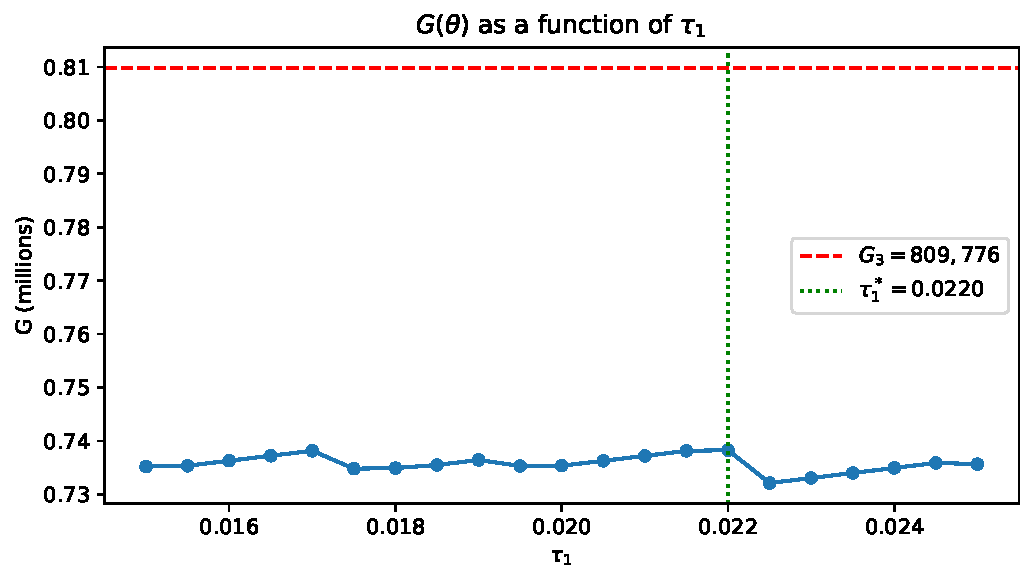
\includegraphics[width=0.65\textwidth]{../figures/q5_tau1_search.pdf}
  \caption{$G(\theta)$ as a function of $\tau_1 \in [0.015,\, 0.3]$ with $\pi_1 = 0.6$ fixed. $G_3 = 811{,}084$ is marked by the dashed line.}
  \label{fig:q5_search}
\end{figure}

$G(\theta)$ is monotonically decreasing in $\tau_1$ throughout the search interval, so the solution is the boundary $\tau_1^* = 0.015$, giving $G(\theta_5^*) = 734{,}557$ (a remaining gap of $76{,}527$ relative to $G_3$). The reform's retirement subsidy creates a highly elastic margin: workers near the employment threshold, already sensitized by $\pi_1 = 0.6$, exit employment when $\tau_1$ rises, shrinking the tax base faster than the higher rate raises per-worker revenue. No $\tau_1$ in this range can restore budget balance.

\paragraph{(c)} We measure individual welfare as realized discounted lifetime utility:
\[
  W_i = \sum_{t=0}^{T-1} \beta^t\, U(c_{i,t},\, l_{i,t}),
\]
where $U$ is as in equation (9). This is computed directly from the simulated consumption and labor-supply paths and is expressed in the same units as the model's value function.

\paragraph{(d)}

\begin{figure}[h!]
  \centering
  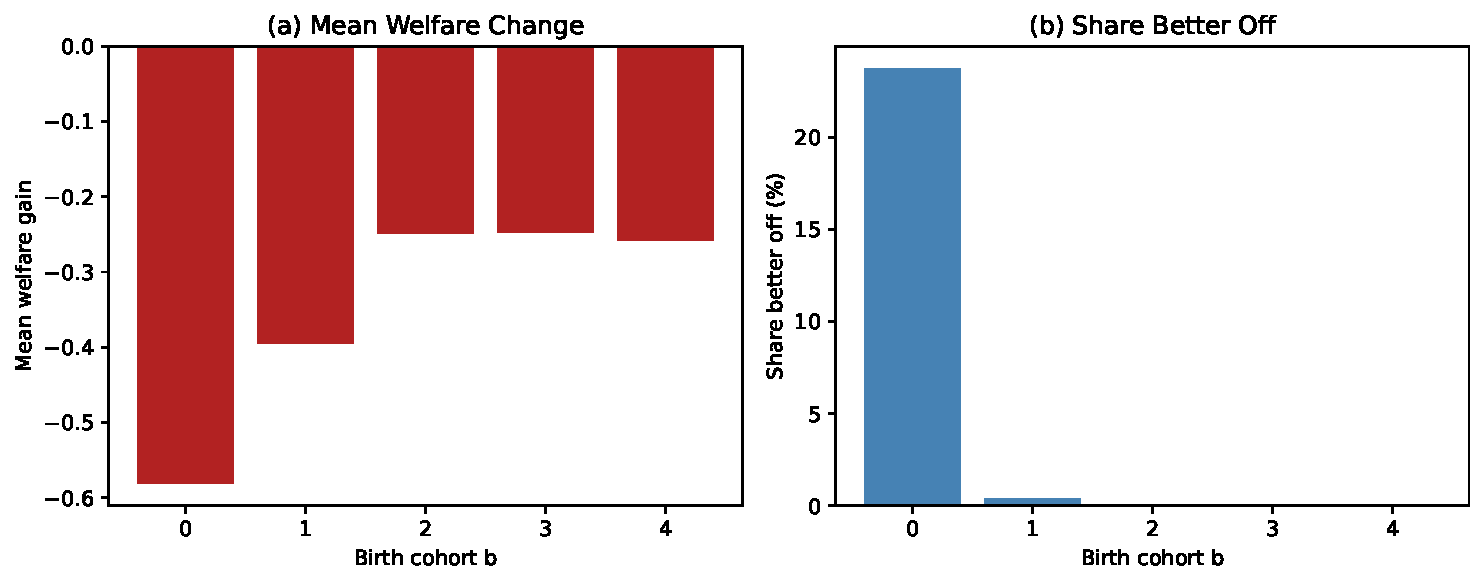
\includegraphics[width=\textwidth]{../figures/q5_welfare_by_cohort.pdf}
  \caption{Welfare analysis by birth cohort under $\theta_5^*$ relative to the baseline. \textit{(a)} Mean welfare gain is negative for all cohorts---the reform is welfare-reducing on average. \textit{(b)} Only cohort $b=0$ has a meaningful share (24.4\%) that is better off; these are the low-wage workers who find it optimal to retire and collect the $\pi_1$ subsidy. Cohorts $b=1$--$4$ have near-zero shares better off ($\leq 0.5\%$), as their higher wages ($\alpha_b$ rises with $b$) make continued employment preferable even after the extra tax.}
  \label{fig:q5_welfare}
\end{figure}

The reform is not Pareto-improving for any cohort. It redistributes toward the lowest-wage workers who switch to retirement, but the additional tax $\tau_1 = 0.015$ combined with the reduced tax base makes the majority of workers worse off. Higher-wage cohorts ($b=2,3,4$) are almost uniformly hurt: they continue to work, pay the extra tax, and receive no subsidy benefit.
